\documentclass[a4paper,11pt]{article}

\usepackage[utf8]{inputenc}
\usepackage[T1]{fontenc}
\usepackage[portuguese]{babel}
\usepackage{graphicx}
\usepackage{geometry}
\usepackage{amsmath}
\usepackage{hyperref}
\geometry{margin=2.5cm}
\usepackage{float}

\title{ProteusTyper: Desenvolvimento de um Algoritmo para Identificação do Locus do Antigénio O em Genomas de \textit{Proteus}}
\author{Carina Ferreira}
\date{}

\begin{document}

\maketitle

\section{Introdução}

O género \textit{Proteus} inclui bactérias Gram-negativas pertencentes à família \textit{Morganellaceae}, sendo amplamente reconhecido pelo seu papel patogénico oportunista, particularmente em infeções do trato urinário \cite{armbruster2012}. Entre as espécies mais relevantes destaca-se \textit{Proteus mirabilis}, frequentemente associada a infeções urinárias complicadas em ambiente hospitalar, sobretudo em doentes com cateterização prolongada.

A crescente prevalência de estirpes bacterianas resistentes a antibióticos reforça a necessidade de desenvolver metodologias robustas para a sua caracterização molecular. Neste contexto, a análise de componentes estruturais como o lipopolissacarídeo (LPS) \cite{raetz2002} assume particular importância. O antigénio O, que corresponde à porção mais variável do LPS, constitui um marcador relevante para tipagem bacteriana, apresentando elevada diversidade genética entre diferentes estirpes.

O locus responsável pela biossíntese do antigénio O encontra-se tipicamente delimitado pelos genes \textit{cpxA} e \textit{secB}. Estudos prévios indicam a existência de aproximadamente 80 serotipos O no género \textit{Proteus} \cite{yu2017}, refletindo a elevada variabilidade desta região genómica. 

Com o avanço das tecnologias de sequenciação de nova geração e o aumento significativo do número de genomas disponíveis em bases de dados públicas, torna-se possível explorar esta diversidade de forma sistemática através de abordagens computacionais. Neste contexto, o desenvolvimento de ferramentas bioinformáticas que permitam a identificação automática deste locus assume particular relevância. Como ilustrado na Figura~\ref{fig:antigenoO}, o antigénio O apresenta elevada variabilidade estrutural, refletindo a diversidade genética desta região.

\begin{figure}[htbp]
    \centering
    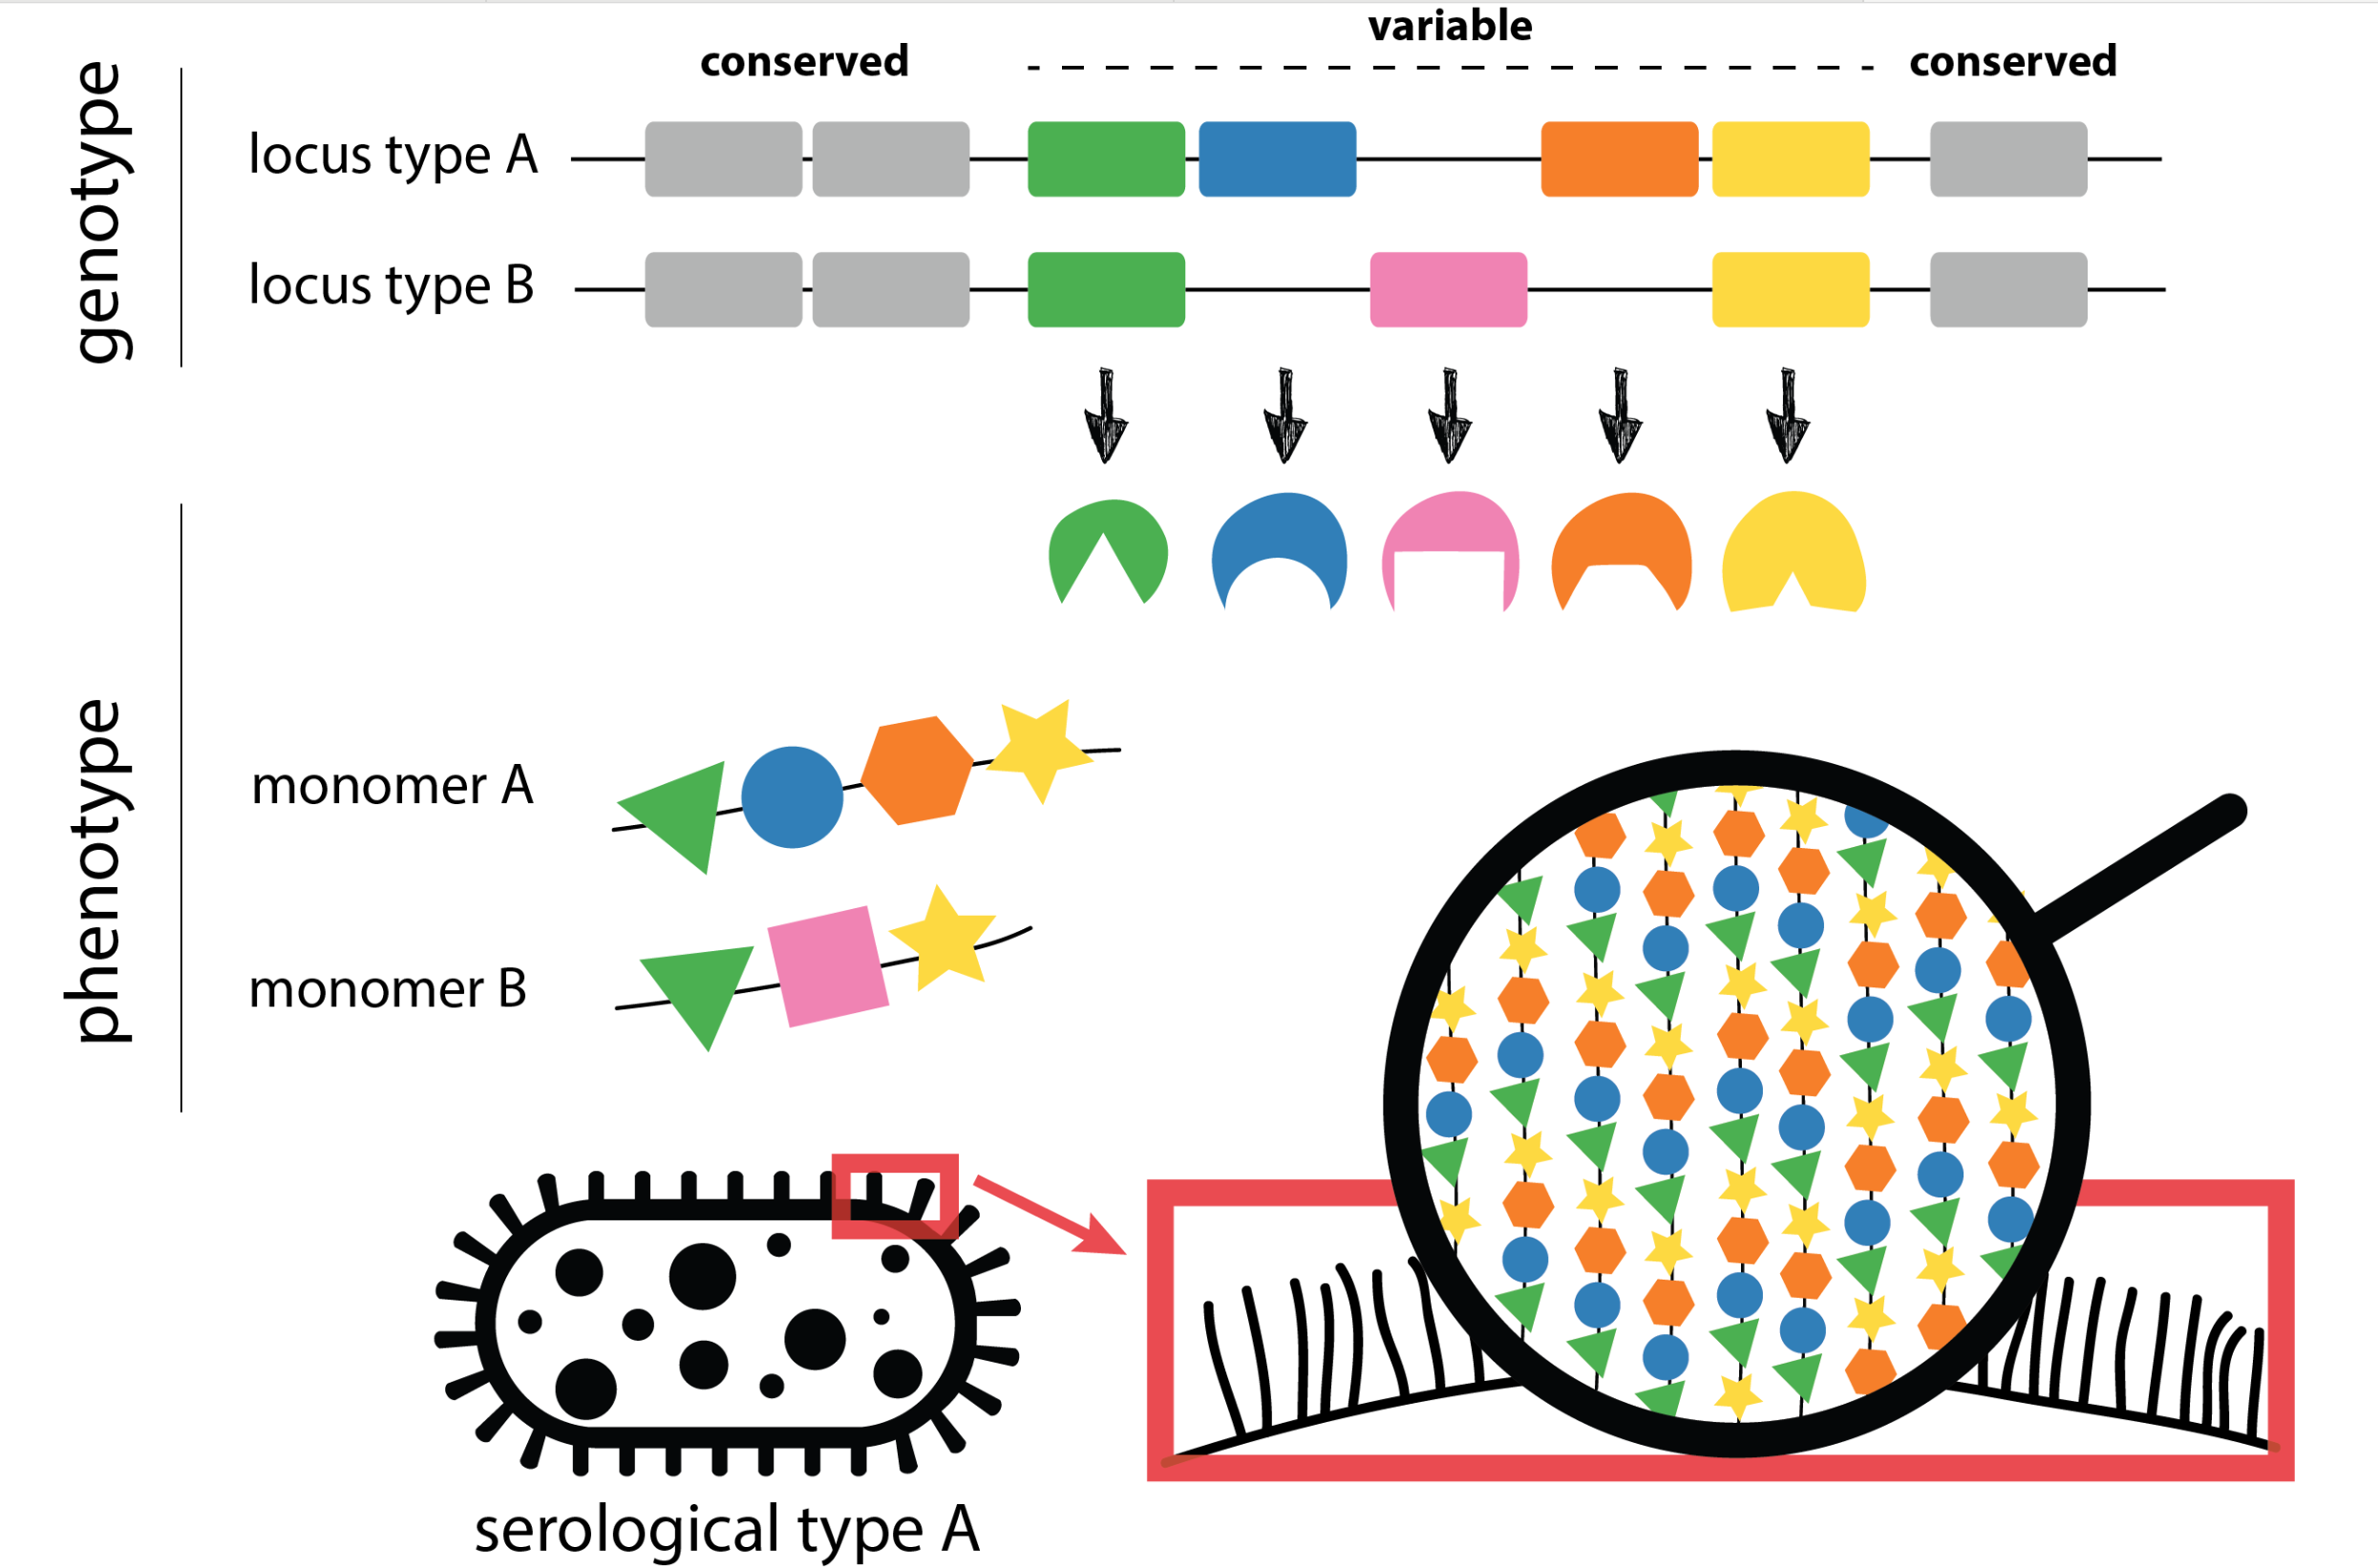
\includegraphics[width=0.65\textwidth]{figura.png}
    \caption{Representação esquemática da biossíntese e diversidade estrutural do antigénio O em bactérias Gram-negativas. Adaptado de material fornecido pelo orientador.}
    \label{fig:antigenoO}
\end{figure}
\clearpage

\section{Estado da Arte}

A tipagem bacteriana evoluiu significativamente com o desenvolvimento das tecnologias genómicas. Métodos tradicionais baseados em características fenotípicas têm vindo a ser progressivamente substituídos por abordagens baseadas na análise de sequências genómicas, permitindo uma caracterização mais precisa e reprodutível.

No caso do género \textit{Proteus}, a diversidade do antigénio O tem sido amplamente estudada, tendo sido descritos cerca de 80 serotipos distintos. A identificação destas variantes foi inicialmente realizada através de métodos experimentais, incluindo técnicas de PCR e análise estrutural.

Adicionalmente, abordagens como o Multi-Locus Sequence Typing (MLST) \cite{maiden1998} permitem a caracterização de estirpes com base na análise de um conjunto de genes housekeeping conservados, sendo amplamente utilizadas em estudos epidemiológicos.

No domínio da bioinformática, diversas ferramentas têm sido desenvolvidas para a identificação automática de loci genómicos. O Kaptive constitui um exemplo relevante \cite{lam2022}, permitindo a identificação de loci capsulares e de LPS através da comparação com bases de dados de referência curadas.

A nível metodológico, a identificação de regiões genómicas pode ser realizada através de diferentes abordagens, incluindo o uso de BLAST para comparação de sequências, HMMER para deteção de genes conservados com base em modelos probabilísticos, e métodos de clustering para agrupamento de sequências semelhantes. Métricas de similaridade, como a percentagem de identidade, são frequentemente utilizadas para classificação de variantes genéticas.

Apesar destes avanços, não existe atualmente uma ferramenta específica para a identificação automatizada do locus do antigénio O em \textit{Proteus}, representando uma lacuna relevante na área.

\subsection{Abordagens Computacionais para Identificação de Loci}

A identificação de loci genómicos em sequências bacterianas baseia-se frequentemente em abordagens de alinhamento e modelação de sequências. Ferramentas como o BLAST permitem identificar regiões homólogas através de alinhamentos locais, sendo amplamente utilizadas para deteção de genes e comparação de sequências.

Por outro lado, métodos baseados em modelos probabilísticos, como o HMMER \cite{eddy2011}, utilizam modelos de Markov ocultos para identificar padrões conservados em sequências, permitindo uma deteção mais sensível de genes mesmo em presença de variação genética significativa.

Adicionalmente, a classificação de variantes genómicas pode ser realizada com base em métricas quantitativas, como a percentagem de identidade e cobertura de alinhamento. Estes critérios são frequentemente utilizados em pipelines bioinformáticos para atribuição de sequências a grupos previamente definidos.

Ferramentas como o Kaptive combinam estas abordagens, permitindo a identificação automática de loci através da comparação com bases de dados curadas \cite{lam2022}, e atribuindo classificações com base em critérios de similaridade. Este tipo de abordagem serve de base conceptual para o desenvolvimento de novas ferramentas aplicadas a diferentes organismos.

\section{Problema Científico}

Embora o locus do antigénio O esteja descrito na literatura científica, a sua identificação em genomas sequenciados ainda não é realizada de forma automatizada e sistemática. Este facto limita a sua aplicação em estudos de larga escala e dificulta a exploração da diversidade genética desta região.

Assim, coloca-se a seguinte questão científica:

\textit{Será possível desenvolver um algoritmo bioinformático eficiente para o calling automático do locus do antigénio O em genomas de \textit{Proteus}, com base na deteção computacional de genes fronteira e na avaliação quantitativa de similaridade entre sequências?}

\section{Objetivos}

\subsection{Objetivo Geral}

Desenvolver um algoritmo bioinformático para a identificação e classificação automática do locus do antigénio O em genomas de \textit{Proteus}.

\subsection{Objetivos Específicos}

\begin{itemize}
    \item Identificar os genes fronteira (\textit{secB} e \textit{cpxA});
    \item Implementar a deteção destes genes com ferramentas como BLAST ou HMMER;
    \item Extrair automaticamente o locus do antigénio O;
    \item Desenvolver um método de classificação baseado em similaridade (ex: identidade >95\%);
    \item Analisar a diversidade genética dos loci obtidos;
    \item Avaliar o desempenho do algoritmo com métricas quantitativas;
    \item Integrar componentes adicionais, como MLST e deteção de genes de resistência.
\end{itemize}

\section{Metodologia Proposta}

O projeto baseia-se no desenvolvimento de um pipeline bioinformático estruturado em várias etapas.

\subsection{Recolha de Genomas}

Serão utilizados genomas completos de \textit{Proteus} disponíveis em bases de dados públicas, nomeadamente no NCBI RefSeq.

\subsection{Deteção de Genes Fronteira}

Os genes \textit{secB} e \textit{cpxA} serão identificados através de anotação genómica ou utilizando ferramentas de alinhamento como BLAST e HMMER.

\subsection{Extração do Locus}

A sequência compreendida entre os genes fronteira será automaticamente extraída, correspondendo ao locus do antigénio O.

\subsection{Classificação do Locus}

As sequências obtidas serão comparadas com uma base de dados de referência. A classificação será realizada com base no melhor alinhamento, utilizando critérios de similaridade, como percentagem de identidade superior a 95\%.

\subsection{Análise de Diversidade}

Será realizada análise comparativa entre loci, incluindo clustering e identificação de variantes, permitindo avaliar a diversidade genética e identificar possíveis novas variantes.

\subsection{Descrição do Algoritmo Proposto}

O algoritmo proposto segue uma abordagem sequencial composta por várias etapas. Inicialmente, é realizada a leitura de genomas anotados em formato GenBank, permitindo aceder à informação estrutural das sequências e à anotação dos genes.

De seguida, procede-se à identificação dos genes fronteira, \textit{secB} e \textit{cpxA}, utilizando pesquisa direta nos ficheiros anotados ou ferramentas de alinhamento como BLAST. Uma vez identificados estes genes, são determinadas as suas posições no genoma.

Com base nas coordenadas obtidas, a sequência compreendida entre estes dois genes é extraída automaticamente, correspondendo ao locus do antigénio O. Esta sequência é então armazenada para análise posterior.

Na fase de classificação, o locus extraído é comparado com uma base de dados de referência, utilizando alinhamentos de sequências. A atribuição de uma variante é realizada com base no melhor alinhamento (best-hit), considerando critérios de similaridade previamente definidos.

Finalmente, os resultados são organizados e apresentados de forma estruturada, permitindo a interpretação dos dados e a identificação de padrões de diversidade genética.

\subsection{Disponibilização}

A ferramenta será disponibilizada através de Google Colab e GitHub, garantindo reprodutibilidade e acessibilidade.

\section{Plano de Trabalho}

O desenvolvimento do projeto será dividido em várias fases ao longo do semestre:

\begin{itemize}
    \item Fase 1 (Semanas 1-2): revisão bibliográfica e definição detalhada do problema;
    \item Fase 2 (Semanas 3-5): desenvolvimento de um protótipo inicial para extração do locus a partir de genomas individuais;
    \item Fase 3 (Semanas 6-8): implementação do algoritmo de classificação baseado em similaridade;
    \item Fase 4 (Semanas 9-11): validação do método com múltiplos genomas e análise de resultados;
    \item Fase 5 (Semanas 12-14): disponibilização da ferramenta e documentação final.
\end{itemize}

Este planeamento permite uma progressão estruturada do projeto, garantindo o desenvolvimento faseado da componente computacional.

\section{Avaliação e Validação do Algoritmo}

A avaliação do algoritmo desenvolvido constitui uma etapa fundamental para garantir a sua robustez e aplicabilidade. Neste contexto, serão utilizados diferentes critérios quantitativos para medir o desempenho da abordagem proposta.

A validação será realizada através da aplicação do algoritmo a um conjunto de genomas de \textit{Proteus} previamente caracterizados, permitindo comparar os resultados obtidos com classificações descritas na literatura. Esta comparação permitirá avaliar a capacidade do algoritmo em identificar corretamente as variantes do locus do antigénio O.

Serão utilizadas métricas como a percentagem de identidade entre sequências, cobertura de alinhamento e consistência dos resultados obtidos. Adicionalmente, será analisada a capacidade do algoritmo em lidar com variações genéticas, incluindo possíveis rearranjos ou inserções no locus.

Outro aspeto relevante será a identificação de casos em que o algoritmo não consiga atribuir uma classificação clara. Estes casos poderão indicar a presença de novas variantes não descritas, sendo alvo de análise adicional.

A avaliação incluirá também a análise do desempenho computacional, nomeadamente o tempo de execução e a escalabilidade da abordagem, aspetos importantes para a sua aplicação em conjuntos de dados de maior dimensão.

Por fim, será considerada a robustez do pipeline face a diferentes formatos de dados e níveis de qualidade das sequências, garantindo a sua aplicabilidade em contextos reais de investigação.

Adicionalmente, serão definidos limiares quantitativos específicos (por exemplo, identidade >95\% e cobertura >90\%) para garantir a consistência e reprodutibilidade do processo de classificação.

\section{Arquitetura do Pipeline Bioinformático}

O sistema proposto poderá ser estruturado sob a forma de um pipeline bioinformático modular, permitindo a execução sequencial das diferentes etapas de análise de forma automatizada e reprodutível.

O pipeline inicia-se com a introdução de um genoma anotado em formato GenBank ou FASTA, que será utilizado como input principal. Numa primeira fase, procede-se à identificação dos genes fronteira, \textit{secB} e \textit{cpxA}, através de métodos de pesquisa baseados em anotação ou alinhamento de sequências.

Após a identificação destes genes, o sistema determina automaticamente as coordenadas correspondentes e extrai a região genómica compreendida entre estes limites, correspondente ao locus do antigénio O.

De seguida, o locus extraído é processado por um módulo de comparação de sequências, que realiza alinhamentos contra uma base de dados de referência previamente construída. Este módulo permite identificar a variante mais próxima, com base em critérios quantitativos como percentagem de identidade e cobertura.

O pipeline inclui ainda um módulo de decisão, responsável pela atribuição da classificação final. Este módulo poderá integrar regras baseadas em limiares definidos (por exemplo, identidade superior a 95\%) e sinalizar casos ambíguos ou potenciais novas variantes.

Os resultados são posteriormente organizados num formato estruturado, incluindo a variante identificada, métricas de similaridade e informação adicional relevante. Estes resultados poderão ser exportados para formatos standard, facilitando a sua integração em análises posteriores.

Por fim, a implementação do pipeline em ambientes como Google Colab permitirá a sua execução de forma acessível e reprodutível, enquanto a disponibilização através de GitHub garantirá transparência e partilha com a comunidade científica.

\section{Conclusão}

O desenvolvimento de um algoritmo bioinformático para a identificação automatizada do locus do antigénio O em \textit{Proteus} permitirá explorar de forma sistemática a diversidade genética desta região. A abordagem proposta integra ferramentas computacionais e critérios quantitativos, garantindo uma metodologia robusta e reprodutível.

Este projeto contribuirá para a criação de soluções bioinformáticas aplicáveis à tipagem genómica, promovendo a sua utilização em contextos de investigação e vigilância epidemiológica.

Adicionalmente, o desenvolvimento deste tipo de ferramentas contribui para a integração de dados genómicos em pipelines automatizados, facilitando a análise de grandes volumes de dados e promovendo a sua utilização em estudos de vigilância epidemiológica e investigação clínica.

\bibliographystyle{plain}
\bibliography{references}

\end{document}